\newcommand{\figureMemoryHierarchy}[1]{
  \def\lang{\detokenize{#1}}
  \def\langRu{\detokenize{ru}}
  \def\langEn{\detokenize{en}}
  \def\figureCaption{XXX: No translation.}
  \ifx \lang\langRu
  \def\figureCaption{
    Иерархия памяти компьютера.
  }
  \fi
  \ifx \lang\langEn
  \def\figureCaption{
    Computer memory hierarchy.
  }
  \fi
  \begin{figure}[H]
    \centering
    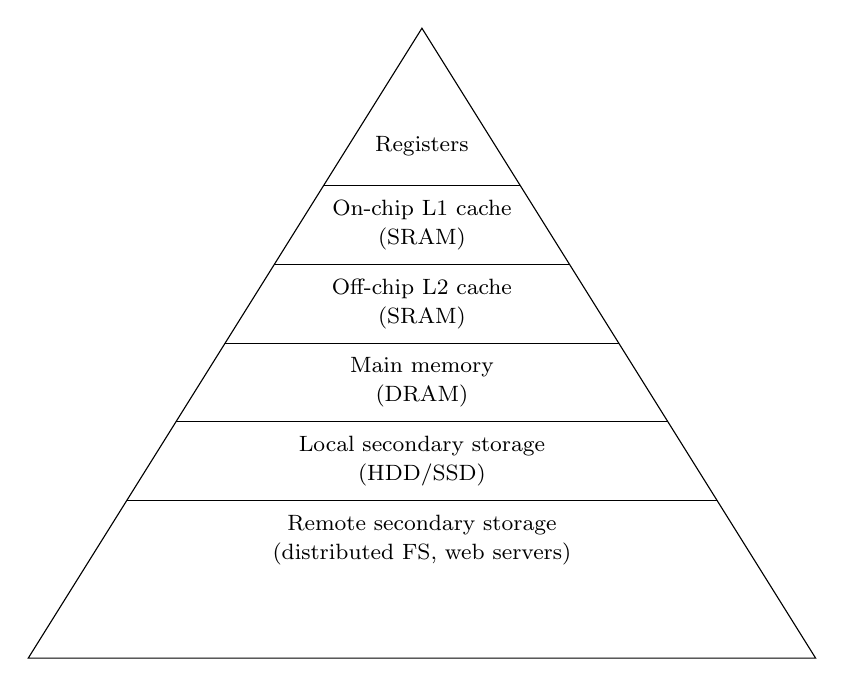
\begin{tikzpicture}
      \draw (5, 8) -- (10, 0) -- (0, 0) -- cycle;
      \foreach \y/\w in {6/1.25, 5/1.88, 4/2.5, 3/3.12, 2/3.75} {
        \draw(5 - \w, \y) -- (5 + \w, \y);
      }
      \draw(5, 6.5) node {
        \footnotesize Registers
      };
      \draw(5, 5.5) node {
        \footnotesize
        \shortstack{On-chip L1 cache\\(SRAM)}
      };
      \draw(5, 4.5) node {
        \footnotesize
        \shortstack{Off-chip L2 cache\\(SRAM)}
      };
      \draw(5, 3.5) node {
        \footnotesize
        \shortstack{Main memory\\(DRAM)}
      };
      \draw(5, 2.5) node {
        \footnotesize
        \shortstack{Local secondary storage\\(HDD/SSD)}
        };
      \draw(5, 1.5) node {
        \footnotesize
        \shortstack{
          Remote secondary storage\\(distributed FS, web servers)
        }
      };
    \end{tikzpicture}
    \caption{\figureCaption}
    \label{fig:memory-hierarchy}
  \end{figure}
}
